\documentclass[11pt,a4paper]{article}
\usepackage[utf8]{inputenc}
\usepackage{hyperref}
\usepackage{minted}
\usepackage{tikz}
\usepackage{graphicx}

\usepackage{todonotes}

\setmintedinline{breaklines}
\setminted{breaklines}

\newcommand{\warning}[1]{
\noindent
\fbox{
\begin{minipage}{0.1\linewidth}
\raisebox{-6em}{
\scalebox{3}{%
\makebox[2.1em][c]{%
\makebox[0pt][c]{\raisebox{0.3em}{\large!}}%
\makebox[0pt][c]{\color{red}\Huge$\bigtriangleup$}}}
}
\end{minipage}
\begin{minipage}{0.1\linewidth}
\hfill
\end{minipage}
\begin{minipage}{0.7\linewidth}
\vspace{1em}
#1
\vspace{1em}
\end{minipage}
\begin{minipage}{0.05\linewidth}
\hfill
\end{minipage}
}
}

\title{Introducing Bluetooth Low Energy}
\author{Kolbjørn Austreng}
\date{}

\begin{document}
\maketitle

\renewcommand{\thesection}{\roman{section}}
\renewcommand{\thesubsection}{\roman{section}.\alph{subsection}}

\section{Introduction}
Wired protocols are all well and nice - and although CAN is a relatively old protocol now partly superseded by CAN-FD (ISO 11898); it is still widely used today. Nevertheless, wireless protocols are becoming increasingly popular wherever they can be used, due to their low cost, and ease of use.\\
\\
One such protocol - Bluetooth Low Energy, or Bluetooth 4.2 (BLE for short) - is almost certainly supported by your smart phone; as well as a plethora of different devices, prevalent in our daily life. This makes it an ideal candidate for introducing wireless connectivity to your project - provided you can live with the interference present in the ISM band.\\
\\
Many of the students taking this course will previously have had the course "Embedded Systems" (TTK4235), in which the "BBC micro:bit" development board was used during the labs. This is an excellent platform for introducing the Bluetooth Low Energy stack, and we will be using the micro:bit platform in this course as well. TTK4235 is no prerequisite, and it should be straight forward to follow this lab assignment without having gone through that course.\\
\\
If no one on your group has a micro:bit, you may talk to one of the student assistants. It is also possible to use other hardware, such as an nRF52 development kit if you happen to have one, but bear in mind that other hardware platforms support different Application Programming Interfaces (APIs) for the Bluetooth stack.

\newpage
\noindent
\section{Initial Setup of Hardward and Toolchain}
The following hardware configuration is only necessary for those of you who have not already done so through TTK4235. However, it might still be necessary to set up the toolchain, as nothing is certain when it comes to the computers at the real time lab.

\subsection{Hardware Configuration}
By default, the micro:bit comes preloaded with a custom Device Abstraction Layer (DAL) that allows programming the device through Scratch, Micropython, or JavaScript. This is well for simple demonstrations, but yields no control of the low level hardware. To get around this limitation, we will upgrade the flasher circuit to use the BBC micro:bit J-Link OB Firmware.

\begin{enumerate}
\item Download the \href{https://www.segger.com/downloads/jlink#BBC\_microbit}{J-Link OB Firmware from Segger.com}\footnote{https://www.segger.com/downloads/jlink\#BBC\_microbit}.
\item Start with the micro:bit unplugged. While holding down the Reset button (next to the USB connector), connect it to the computer.
\item The micro:bit should now have mounted itself as "MAINTENANCE" on the file system. You can now let go of the Reset button.
\item Move the .hex-file that you downloaded into "MAINTENANCE".
\item The micro:bit should now automatically remount after a few seconds; this time as "MICROBIT".
\end{enumerate}

\subsection{Toolchain Configuration}
\label{sec::toolchain_config}
To compile and flash code for the micro:bit, we need to install a toolchain. For compilation, GCC is a natural choice. Since the heart of the micro:bit is an nRF51822, we will be using J-Link and nrfjprog to flash the board.

\begin{enumerate}
\item Call \mintinline{text}{nrfjprog --version} to see if the toolchain is already set up on the computer. If it is, you may skip the remaining steps.
\item Call \mintinline{text}{sudo apt install gcc-arm-none-eabi} to install the GCC ARM compiler.
\item Go to \href{https://www.nordicsemi.com/eng/nordic/Products/nRF51822/nRF5x-Command-Line-Tools-Linux64/51386}{nordicsemi.com}\footnote{https://www.nordicsemi.com/eng/nordic/Products/nRF51822/nRF5x-Command-Line-Tools-Linux64/51386} and download the newest version of the nRF command line tools.
\item The download contains the programs \mintinline{text}{nrfjprog} and \mintinline{text}{mergehex}, both must be available in the Linux \mintinline{text}{PATH} variable. This can be done in many ways, here is one:
\begin{enumerate}
\item Extract the \mintinline{text}{nrfjprog}- and \mintinline{text}{mergehex} folders to the home folder.
\item Add the following string at the bottom of the \mintinline{text}{~/.bashrc} file: \mintinline{bash}{"export PATH=$HOME/nrfjprog:$HOME/mergehex:$PATH"} (do not include the quotation marks)%$
\item Finally, since \mintinline{text}{~/.bashrc} is read once when a terminal opens, you need to close and reopen all terminal windows that you might have active.
\end{enumerate}
\item Go to \href{https://www.segger.com/downloads/jlink/\#J-LinkSoftwareAndDocumentationPack}{segger.com}\footnote{https://www.segger.com/downloads/jlink/\#J-LinkSoftwareAndDocumentationPack} and download the J-Link Software and Documentation pack. You should choose the Linux 64 bit version, DEB installer.
\item Once you have downloaded the DEB package, navigate to the download location with a terminal, and call the following command to install the package: \mintinline{text}{sudo dpkg -i JLink_Linux[...]x86_64.deb}
\end{enumerate}

\subsection{Hardware and Toolchain Verification}
First off, you should call \mintinline{text}{nrfjprog --version} to see if the toolchain is set up. If this command complains, you will need to repeat section \ref{sec::toolchain_config}.\\
\\
On Blackboard, you can find an example .hex-file, aptly named "example.hex". To flash this file to the micro:bit, navigate to the directory where you have the hex, and call:
\begin{minted}{bash}
nrfjprog -f nrf51 --chiperase --program example.hex --reset
\end{minted}
The micro:bit should now start broadcasting the name "u:bit" over Bluetooth. To verify this, you may use your phone, as described in section \ref{sec::phone_verify}.

\section{Use your phone for testing}
\label{sec::phone_verify}
You are free to use whatever to check your Bluetooth connection, but an easy choice is to download the "nRF Connect" app for your smart phone. This lab assignment will use that app.\\
\\
When you open nRF Connect, your phone will start scanning for advertising packets, as seen in figure \ref{fig::example_scanning}. You can adjust the RSSI filter (signal strength) to only show devices that are close to you. In the image, this filter is set to $-80$ dBm, but setting it to around $-60$ dBm is probably better if there are a lot of Bluetooth devices nearby.\\
\\
When you connect to the micro:bit, you will see something similar to figure \ref{fig::example_services}. The names "LED Matrix" and "Buttons" will not show up by default, but may be assigned by you, by long-pressing on the \textit{characteristic} and editing the name. Either way, the name of the characteristic is merely cosmetic.\\
\\
By uploading a byte different than 0x00 to the "LED Matrix" characteristic, the LED matrix should turn on; and it should turn off when you upload 0x00.\\
\\
The "Buttons" characteristic contains the state of the two micro:bit tactile buttons. You may read their state \textit{once} by pressing the download icon - or you may \textit{subscribe} to state updates by pressing the "notify" icon (The solid line with three arrows pointing down). With subscriptions turned on, you should see the state of the buttons update on the screen as you press- and release the buttons.

\begin{figure}[ht]
\centering
\begin{minipage}{0.5\linewidth}
\centering
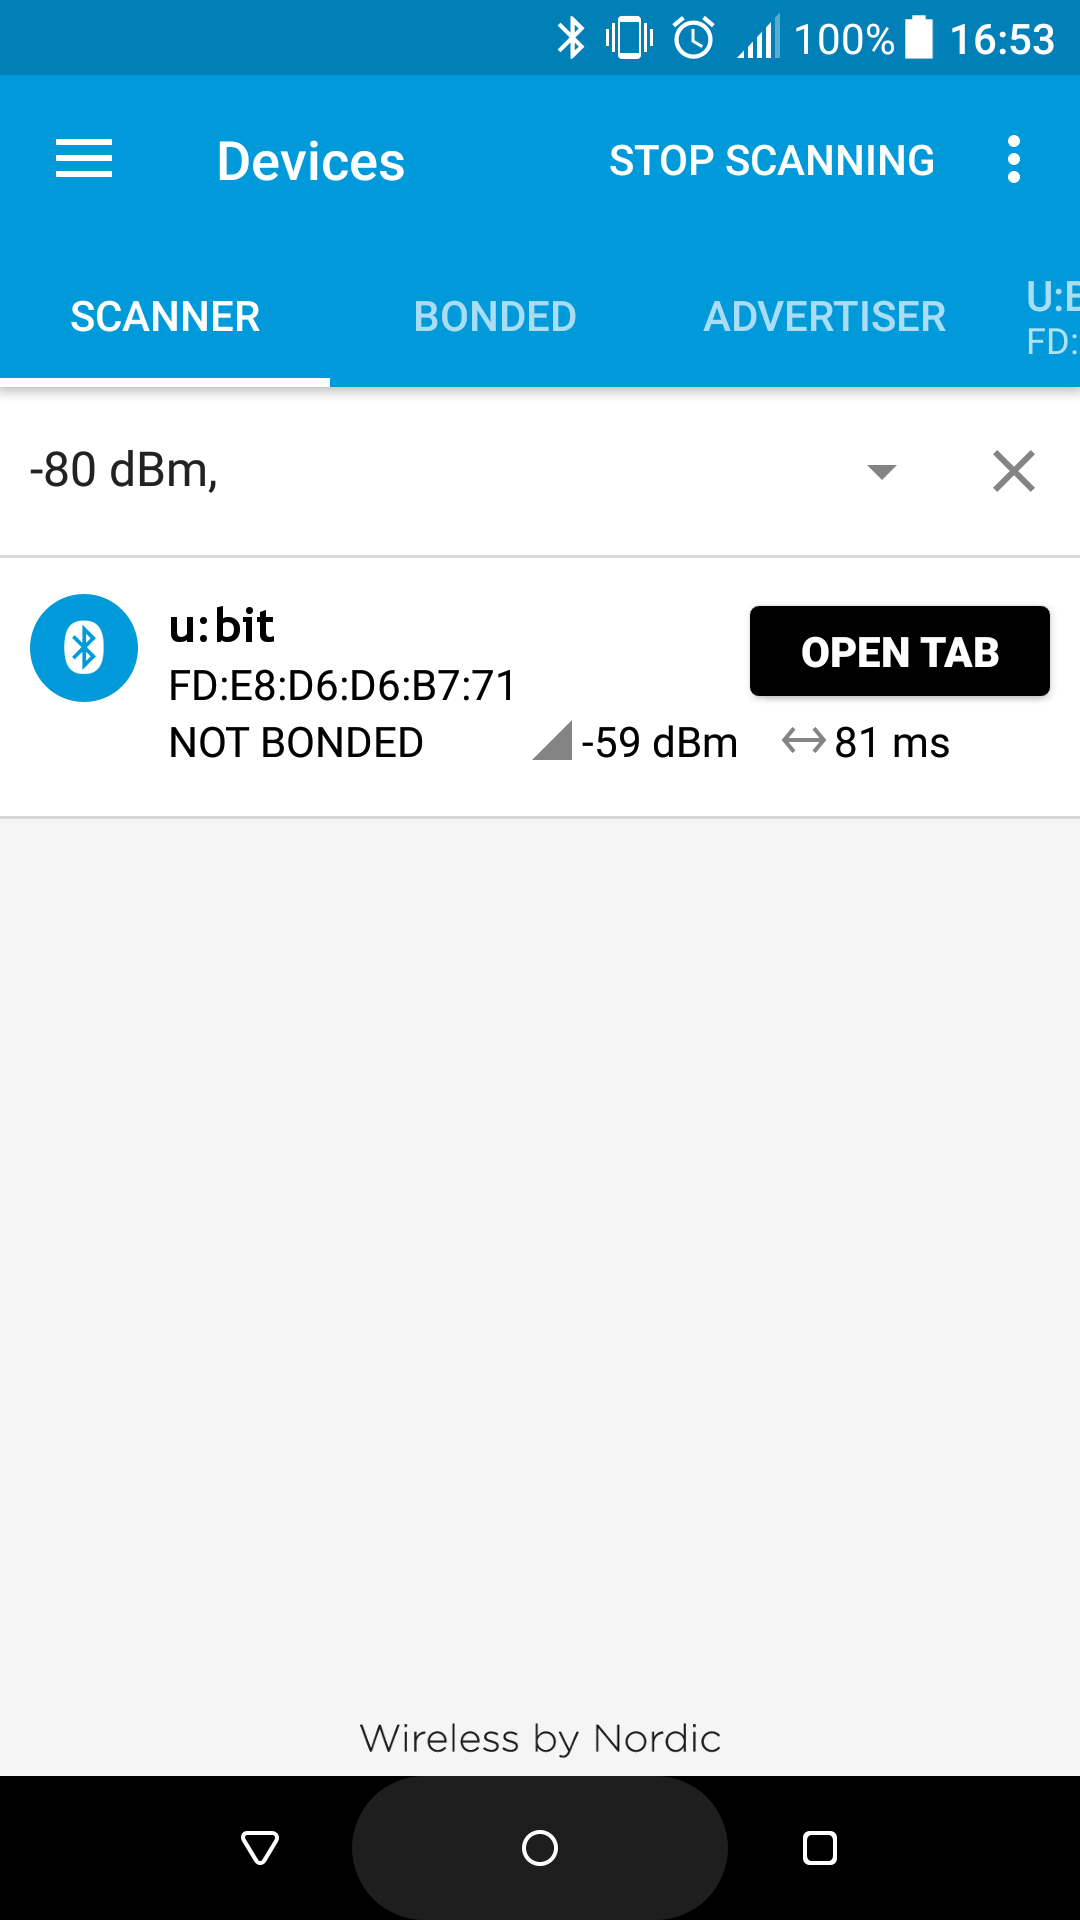
\includegraphics[width=0.9\linewidth]{example_connect_scan.png}
\caption{nRF Connect scanning.}
\label{fig::example_scanning}
\end{minipage}%
\begin{minipage}{0.5\linewidth}
\centering
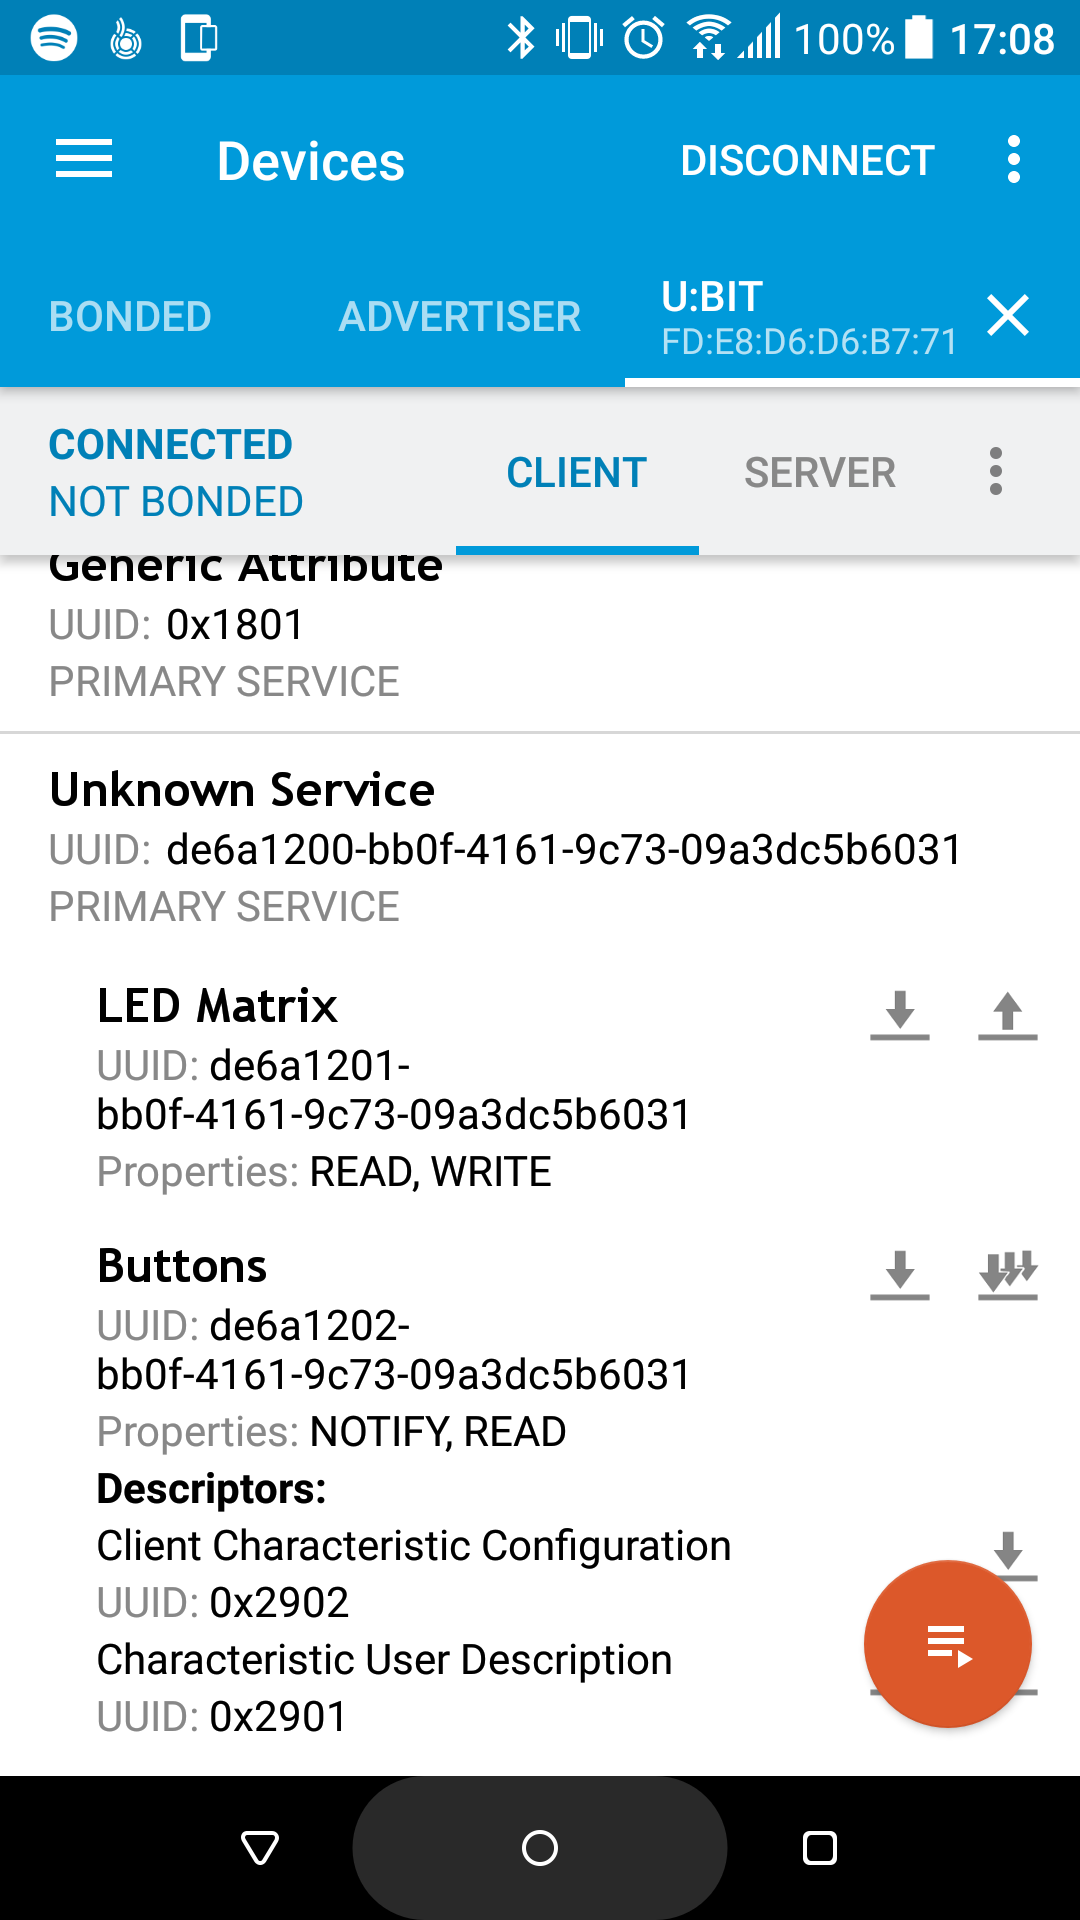
\includegraphics[width=0.9\linewidth]{example_connect_gatt.png}
\caption{Example services.}
\label{fig::example_services}
\end{minipage}
\end{figure}

\newpage
\noindent
\setcounter{section}{0}
\renewcommand{\thesection}{\arabic{section}}
\renewcommand{\thesubsection}{\arabic{section}.\arabic{subsection}}

\section{Heads up}
Bluetooth Low Energy (BLE) is a messy beast to tackle, so it might be smart to skim appendix \ref{app::intro_ble} as you go through this lab assignment. Don't fret if you do not get all the details however - some things are better understood when coded, rather than when read.\\
\\
Finally, an honest word from the author of this assignment: Sometimes, the Nordic Semi documentation can be a little "Meh". Feeling like there should be a more elegant way to do Bluetooth Low Energy is completely normal - and you are advised to simply bite the pillow when the going gets rough.\\
\\
Do enjoy :)

\section{First steps - GAP}
The gatekeeper of Bluetooth is the \textit{Generic Access Profile}. This is the part of Bluetooth that handles broadcasting, discovery, the setting up- and managing connections, as well as negotiating security levels.\\
\\
Although GAP is used to establish connections, GAP itself is connectionless, and pretty simple. The bottom line is this: When advertising, a Bluetooth device sends out an \textit{Advertising Packet} of 31 bytes every advertising interval - which can be anything between $20$ milliseconds and $10.24$ seconds.\\
\\
In addition to this, anyone observing the advertiser can send a \textit{scan request} to the device. Upon receiving such a scan request, the device \textit{may} respond with a \textit{Scan Response Packet}, which is also 31 bytes and can contain different information than the Advertising Packet. Note that the device is not required to respond to scan requests, however.\\
\\
GAP happens entirely on the Bluetooth channels 37, 38, and 39, which are reserved for advertising - as illustrated in figure \ref{fig::bluetooth_spectrum} in appendix \ref{app::intro_ble}. The reason that exactly these channels were chosen for advertising is to avoid most of the interference from WiFi, which is most noticeable on the channels 0-9, 11-20, and 23-32.\\
\\
To make matters a little more interesting, the Bluetooth 4.2 specification specifies 4 different ways a device can advertise. The nuances of this is not terribly important for this course, but they are listed here for the interested:
\begin{itemize}
\item \mintinline{text}{ADV_IND}: "Connectable undirected advertising". This is the regular way to advertise. Any other device can request a scan response or a connection.
\item \mintinline{text}{ADV_DIRECT_IND}: "Connectable directed advertising". This is used to ask a specific central for a connection. The packet is a broadcast packet, but scanners will ignore it if the peer address does not match them. In addition, the advertiser itself will ignore all scan requests.
\item \mintinline{text}{ADV_SCAN_IND}: "Scannable undirected advertising". In this mode, the advertiser will ignore all connection requests, but may respond to scan requests.
\item \mintinline{text}{ADV_NONCONN_IND}: "Non-connectable undirected advertising". This is essentially just an information beacon; the advertiser will ignore all scan- and connection requests, and will simply spew out its own Advertising Packets until the end of time.
\end{itemize}

\subsection{Advertising Packet Format}
Even though the Advertising Packet (and Scan Response Packet) consists of 31 bytes, not all are usable by the application programmer. This is because the packet is subdivided into a number of \textit{AD Structs} - or "Advertising Data Structures". Actually, truth be told, each Advertising Packet may \textit{really} send out 47 bytes over the air each advertising interval, but a lot of this is overhead, as illustrated in figure \ref{fig::pdu_breakdown}. The squares with just numbers in them denote fields that are necessary, but not of direct interest to us.\\
\begin{figure}[ht]
\centering
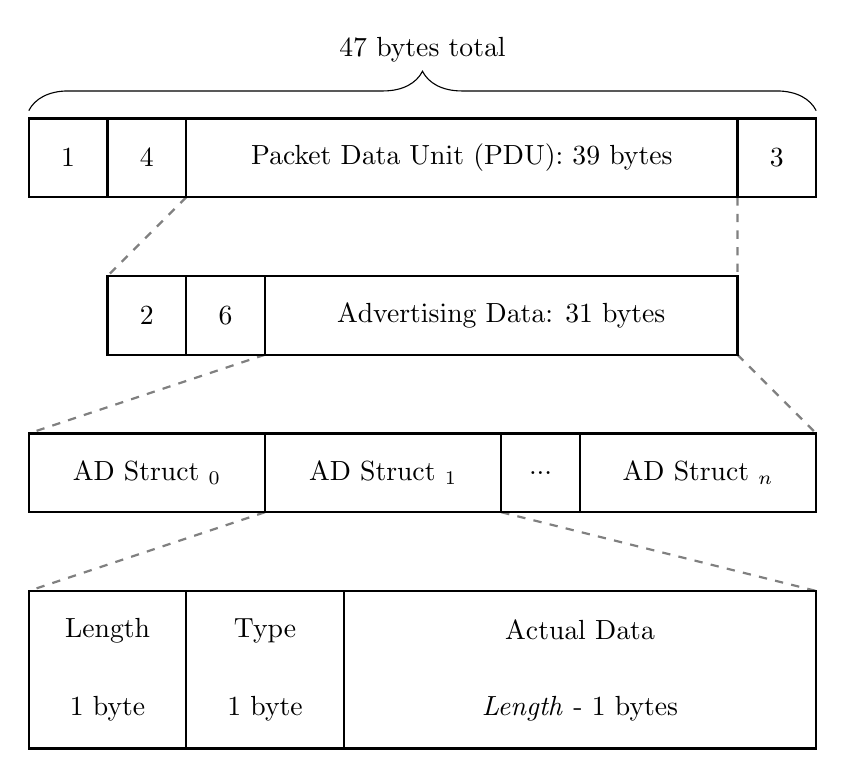
\begin{tikzpicture}
%\draw[gray!35] (0,0) grid (10,-7);
\usetikzlibrary{decorations.pathreplacing}

\draw[decoration={brace,amplitude=5mm}, decorate, yshift=0.1cm] (0,0) -- ++(10,0)
node[midway, above=0.5cm] {47 bytes total};

\draw[gray,dashed,thick] (2,-1) -- +(-1,-1) ++ (7,0) -- ++(0,-1)
++(0,-1) -- +(1,-1) ++(-6,0) -- ++(-3,-1) ++(3,-1) -- +(-3,-1) ++(3,0) -- ++(4,-1);

\draw[thick] (0,0) rectangle ++(1,-1) node[midway] {1}
rectangle ++(1,1)  node[midway] {4} 
rectangle ++(7,-1) node[midway] {Packet Data Unit (PDU): 39 bytes}
rectangle ++(1,1) node[midway] {3};

\draw[thick] (1,-2) rectangle ++(1,-1) node[midway] {2}
rectangle ++(1,1) node[midway] {6}
rectangle ++(6,-1) node[midway] {Advertising Data: 31 bytes};

\draw[thick] (0,-4) rectangle ++(3,-1) node[midway] {AD Struct $_0$}
rectangle ++(3,1) node[midway] {AD Struct $_1$}
rectangle ++(1,-1) node[midway] {...}
rectangle ++(3,1) node[midway] {AD Struct $_n$};

\draw[thick] (0,-6) rectangle ++(2,-2) rectangle ++(2,2) rectangle ++(6,-2);
\path (0,-6) rectangle ++(2,-1) node[midway] {Length}
rectangle ++(2,1) node[midway] {Type}
rectangle ++(6,-1) node[midway] {Actual Data};
\path (0,-7) rectangle ++(2,-1) node[midway] {1 byte}
rectangle ++(2,1) node[midway] {1 byte}
rectangle ++(6,-1) node[midway] {\textit{Length} - 1 bytes};

\end{tikzpicture}
\caption{Breakdown of each GAP advertising transmission unit.}
\label{fig::pdu_breakdown}
\end{figure}\\
Despite the fact that we do not really get to use all the 31 bytes in the advertising data, we must still hand craft the entire field to comply with with the Bluetooth 4.2 spec in our code. In fact, you can see the advertising data used in the example program in listing \ref{code::example_advertise_data}.\\
\begin{listing}[hb]
\begin{minted}{c}
static uint8_t adv_data[] = {
	6, BLE_GAP_AD_TYPE_COMPLETE_LOCAL_NAME,
	'u', ':', 'b', 'i', 't',
	3, BLE_GAP_AD_TYPE_16BIT_SERVICE_UUID_COMPLETE,
	0x0D, 0xF0
};
uint8_t adv_data_length = 11;
\end{minted}
\caption{The advertising data field from the example hex.}
\label{code::example_advertise_data}
\end{listing}\\
Note that the advertising data does not have to use all the 31 bytes available. We are free to use fewer bytes, and therefore transmit less data over the air each advertising interval. This allows us to reduce power consumption a little if we have a really resource constrained application.

\subsection{Write the code}
You have already been handed out some C-files that you may build on. If you happen to be a masochist, you are of course free to discard this code and start from scratch. Otherwise, follow along.\\
\\
In the \mintinline{text}{main} function, you will see a call to \mintinline{text}{bluetooth_init()}. This is simply a wrapper around two calls to first initialize the Nordic SoftDevice, before enabling the Bluetooth Low Energy stack with some sane parameters. You do not need to worry about this; instead, you will be implementing the \mintinline{text}{bluetooth_gap_advertise_start()} function, which is responsible for setting up the AD structs (figure \ref{fig::pdu_breakdown}), and then enabling advertising.\\
\\
The first step is to open up the documentation for the Nordic SoftDevice. Open up \mintinline{text}{softdevice/s130_nrf51_2.0.1_API/html/index.html} in a web browser. From there, navigate to the \mintinline{text}{Modules} tab, then click \mintinline{text}{Generic Access Profile (GAP)}, and then click on \mintinline{text}{Functions}.\\
\\
You will now be greeted with a fairly intimidating looking list of things. If you are feeling a little bit overwhelmed at this point, read section \ref{sec::what_on_earth}. If you are feeling confident, feel free to skip ahead.

\subsubsection{What on earth is all this?}
\label{sec::what_on_earth}
Most of the documentation for the Nordic SoftDevices is handed out as specially formatted comments in the header files of the SoftDevice API. You can then generate a more friendly format, such as an HTML web site, using a handy program called \mintinline{text}{doxygen}. This has already been done for you, but it is pretty easy to do yourselves as well.\\
\\
Doxygen is very handy for integrating documentation into code, and often leads to more up to date documentation in general. The only flip side is that the output is slightly less human friendly than it would otherwise have been, had it been hand crafted by an actual human being. Do not despair though, let us dissect this cryptic output together:

\begin{figure}[h]
\centering
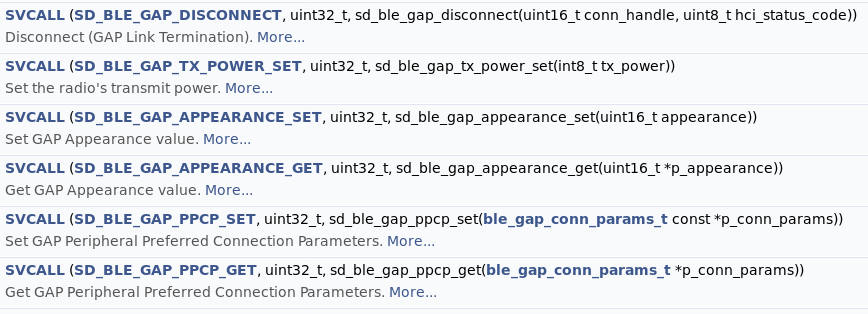
\includegraphics[width=0.9\linewidth]{softdevice_documentation_example.png}
\caption{SoftDevice GAP documentation except.}
\label{fig::gap_documentation_excerpt}
\end{figure}

\noindent
In figure \ref{fig::gap_documentation_excerpt}, you can see an excerpt of the SoftDevice GAP documentation. Each line starts with the macro \mintinline{text}{SVCALL} - which stands for "\mintinline{text}{Supervisor Call}". This is simply an implementation detail, and not something that we have any control over.\\
The actual function that we want to call is listed after this macro. For example, in the line \mintinline{text}{SVCALL(SD_BLE_GAP_TX_POWER_SET, uint32_t [...])}, the function that is available to us is called

\begin{minted}{c}
sd_ble_gap_tx_power_set(int8_t tx_power);
\end{minted}

\noindent
Underneath the \mintinline{text}{SVCALL} line, you can see a short description of what this function does, along with a link that will give you more detailed information about how you should use the function.\\
\\
Many functions will take a pointer to a custom defined struct, instead of several smaller parameters. This is again due to implementation details. In some such cases, the memory that the pointer points to, must remain available after the function has executed. In those cases, manually allocating memory or marking the variable as static is recommended.\\
\\
Finally, it might be worth pointing out some of the coding standard used in the SoftDevice public API:
\begin{enumerate}
\item There is liberal use of the \mintinline{c}{const} keyword, to signal the compiler that a variable should not be changed. This is good practice - especially when dealing with things that can easily break, such as Bluetooth code.
\item Pointer variables are always prefixed with \mintinline{text}{p_}, and in the rare cases of pointer-to-pointer, the prefix \mintinline{text}{pp_} is used. This is heartily recommended, as it is a quick way to kill off some otherwise hard-to-find bugs.
\item In the documentation of each function, the parameters will be marked with either \mintinline{text}{[in]}, \mintinline{text}{[out]}, or \mintinline{text}{[in,out]}. This tells you whether the function intends to modify the input parameter or not. Parameters marked \mintinline{text}{[in]} will not be modified, whereas \mintinline{text}{[out]} and \mintinline{text}{[in,out]} will.
\end{enumerate}

\subsubsection{Set the advertising data}
The first step you need to do is setting the Advertising Packet data content. In the \mintinline{text}{bluetooth.c} file, you will find an incomplete function called \mintinline{text}{bluetooth_gap_advertise_start()}. Your task is to fill out the \mintinline{c}{static uint8_t adv_data[]} array with data according to one or more AD structs, as illustrated in figure \ref{fig::pdu_breakdown}.\\
\\
The function of most interest to you is called \mintinline{text}{sd_ble_gap_adv_data_set}. You are free to skip the Scan Response Packet, in which case you simply set \mintinline{text}{p_sr_data} to \mintinline{c}{NULL}, and \mintinline{text}{srdlen} to \mintinline{c}{0}.\\
\\
For a complete list of the AD Struct types that this SoftDevice supports, you may check out \mintinline{text}{Generic Access Profile (GAP)} $\rightarrow$ \mintinline{text}{Defines} $\rightarrow$ \mintinline{text}{GAP Advertising and Scan Response Data format}.

\warning{If you are interested in using both a complete local name, as well as short local name, there is one caveat you need to be aware of: A short local name must be a continuous subset of the complete local name, starting at the beginning of the complete name - as per the Bluetooth Core Specification Supplement version 7. No worries, it took me ages to figure out as well.}

\subsubsection{Start advertising}
After you have set the advertising data, you need to activate advertising. Check out the documentation for \mintinline{text}{sd_ble_gap_adv_start}. Note that this function call takes a pointer to a \mintinline{text}{ble_gap_adv_params_t} struct.\\
\\
To get the fields of this struct, follow the link in the documentation of the \mintinline{text}{sd_ble_gap_adv_start} function. New tabs for each link you have to follow is advisable, but remember to close the ones you no longer need - otherwise you \textit{will} be overrun with information quickly.\\
\\
Hint: Only the fields \mintinline{text}{type} and \mintinline{text}{interval} are of particular interest, while the rest of the struct can be all zeros. A neat way to do this without manually setting each field is using the \mintinline{c}{memset} function, provided by \mintinline{c}{<string.h>}:

\begin{minted}{c}
ble_gap_adv_params_t adv_params;
memset(&adv_params, 0, sizeof(adv_params));
// Then set only the interesting fields
\end{minted}
To get the documentation for \mintinline{c}{memset}, you may call \mintinline{text}{man 3 memset} in a terminal, but the long and short of it is this: Fill \mintinline{c}{sizeof(adv_params)} number of bytes with all zeros, starting at the address of \mintinline{text}{adv_params}.\\
\\
You stand free to choose the advertising type, but you are most likely interested in using \mintinline{text}{BLE_GAP_ADV_TYPE_ADV_IND}. You can find a complete list of advertising types under \mintinline{text}{Generic Access Profile (GAP)} $\rightarrow$ \mintinline{text}{Defines} $\rightarrow$ \mintinline{text}{GAP Advertising types}.

\subsection{Print to check your code}
All the SoftDevice calls will return 0 (which is the value of\mintinline{text}{NRF_SUCCESS}) upon successful execution. You can print this over UART to the computer by using the provided \mintinline{text}{ubit_uart_print} function - which works the same way \mintinline{text}{printf} does, except that \mintinline{text}{ubit_uart_print} only accepts integers. An example invocation looks like this:
\begin{minted}{c}
ubit_uart_init(); // Call once
ubit_uart_print("My favorite number is %d\n\r", 2);
\end{minted}
To read the micro:bit UART output, you may use any serial terminal program that you choose, with the baudrate 9600. The micro:bit will most likely mount as \mintinline{text}{/dev/ttyACM0}. An example using the \mintinline{text}{picocom} program looks like this:
\begin{minted}{text}
picocom -b 9600 /dev/ttyACM0
\end{minted}
\warning{If you have any other USB UART interfaces connected to the computer, the micro:bit may mount as \mintinline{text}{/dev/ttyACM1} instead. You can call \mintinline{text}{dmesg --follow} and then connect the micro:bit if you want to be sure where it mounts.}

\subsubsection{Check with your phone}
If your program compiles and runs, you may check with your phone to see if there is anything on the air. Use the nRF Connect app and start scanning. Your micro:bit should now broadcast its name, along with any other AD Structs that you might have included.\\
\\
If you made it, take a moment to savor your victory; writing Bluetooth Low Energy firmware is not a trivial task ;)\\
\\
Note that if you try to connect to your micro:bit at this point, you will be met with very anticlimactic behavior: The default when a device is attempted connected to, is to stop advertising. However, since we have not implemented any connection acceptance yet, the device will simply turn off advertising and then idle - and then your phone will time out.\\
\\
Finally, you might have noticed that the nRF Connect app reports a different advertising interval than you specified. For example, if you chose 80 ms in your code, you will typically see an actual advertising interval of around 85 ms. This is because the Bluetooth spec will add a random delay to the specified interval, in order to reduce the likelihood of packet collisions.




\newpage
\noindent
\appendix
\section{Introduction to BLE}
\label{app::intro_ble}
\begin{figure}
\centering
\resizebox{\linewidth}{!}{
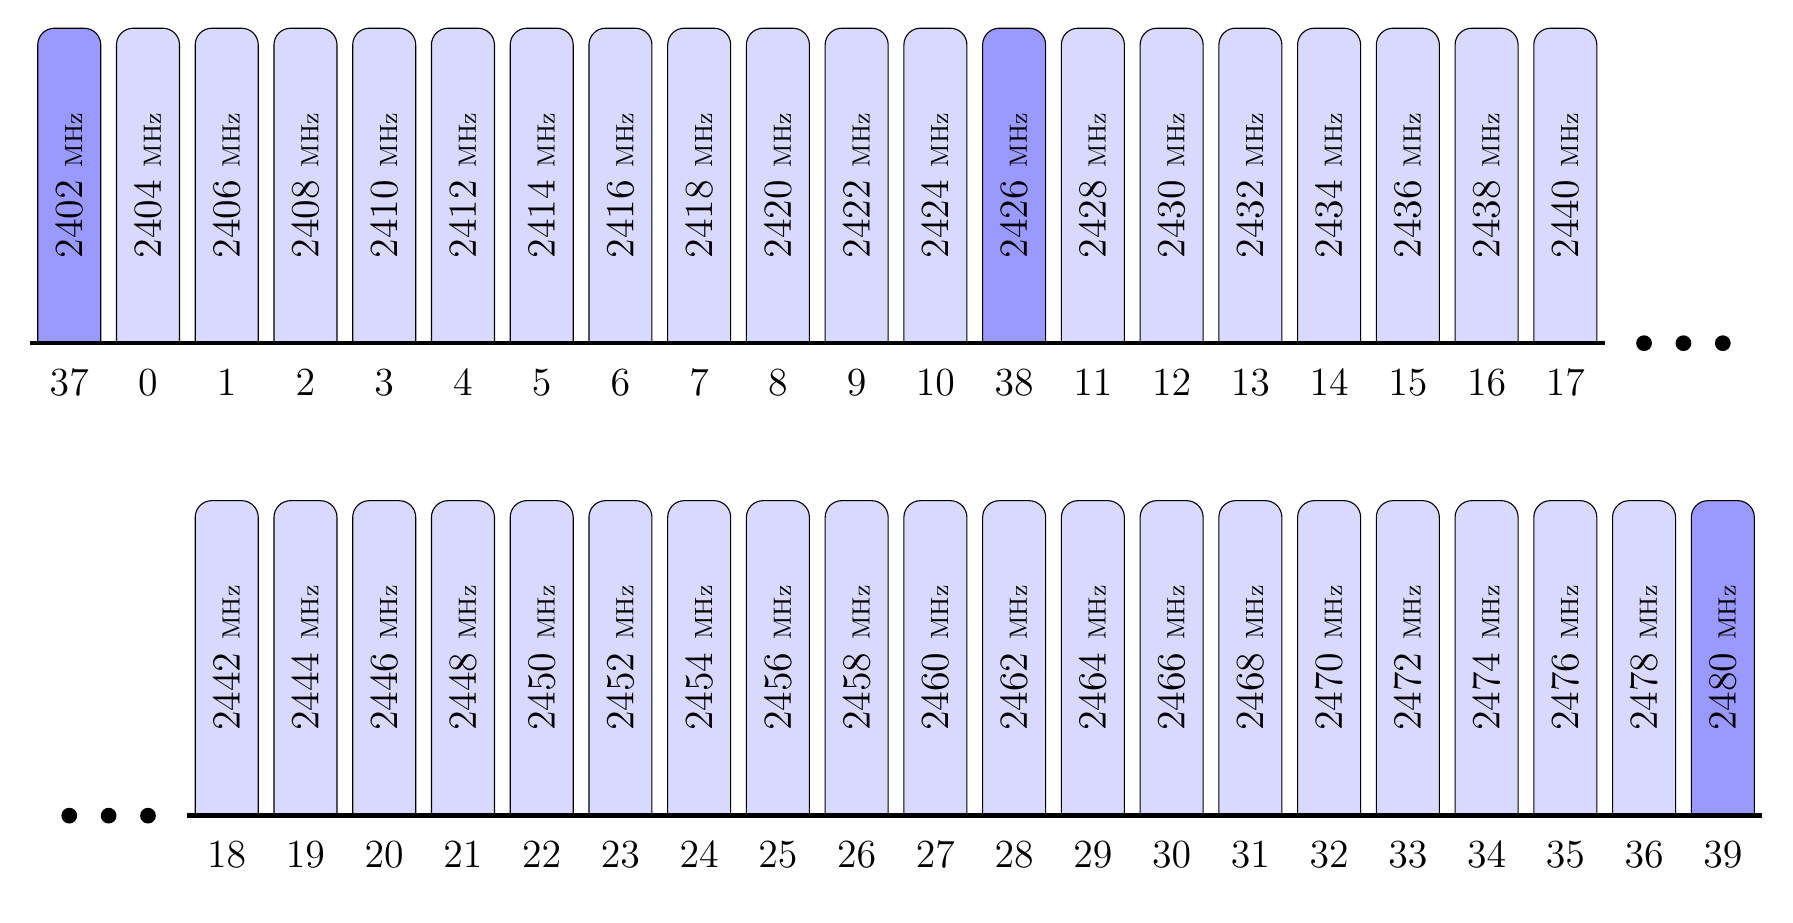
\begin{tikzpicture}
%\draw[gray] (0,0) grid (10,4);

\colorlet{regular_channel_fill}{blue!15}
\colorlet{advertise_channel_fill}{blue!40}

\foreach \x in {0,1,...,19}{
\fill[regular_channel_fill,rounded corners=0.6em](\x + 0.1, 0) -- ++(0,4) -- ++(0.8,0) -- ++(0,-4);
}
\foreach \x in {0,12}{
\fill[advertise_channel_fill,rounded corners=0.6em](\x + 0.1, 0) -- ++(0,4) -- ++(0.8,0) -- ++(0,-4);
}
\foreach \x in {0,1,...,19}{
\pgfmathsetmacro{\f}{int(2402 + 2 * \x)}
\draw[rounded corners=0.6em] (\x + 0.1,0) -- ++(0,4) -- ++(0.8,0) -- ++(0,-4);
\path (\x,0) rectangle ++(1,4) node[midway,rotate=90] {\Large$\f$ \small MHz};
}
\foreach \x/\ch in {0/37,1/0,2/1,3/2,4/3,5/4,6/5,7/6,8/7,9/8,10/9,11/10,12/38,13/11,14/12,15/13,16/14,17/15,18/16,19/17}{
\path (\x,-1) rectangle ++(1,1) node[midway] {\Large\ch};
}
\draw[ultra thick] (0,0) -- ++(20,0);
\foreach \x in {1,1.5,2}{
\fill (19.5 + \x, 0) circle [radius=0.1];
}

% Line two
\begin{scope}[xshift=-18cm, yshift=-6cm]
\foreach \x in {20,21,...,39}{
\fill[regular_channel_fill,rounded corners=0.6em](\x + 0.1, 0) -- ++(0,4) -- ++(0.8,0) -- ++(0,-4);
}
\fill[advertise_channel_fill,rounded corners=0.6em](39 + 0.1,0) -- ++(0,4) -- ++(0.8,0) -- ++(0,-4);
\foreach \x in {20,21,...,39}{
\pgfmathsetmacro{\f}{int(2402 + 2 * \x)}
\draw[rounded corners=0.6em] (\x + 0.1,0) -- ++(0,4) -- ++(0.8,0) -- ++(0,-4);
\path (\x,0) rectangle ++(1,4) node[midway,rotate=90] {\Large$\f$ \small MHz};
}
\foreach \x/\ch in {20/18,21/19,22/20,23/21,24/22,25/23,26/24,27/25,28/26,29/27,30/28,31/29,32/30,33/31,34/32,35/33,36/34,37/35,38/36,39/39}{
\path (\x,-1) rectangle ++(1,1) node[midway] {\Large\ch};
}
\draw[ultra thick] (20,0) -- ++(20,0);
\foreach \x in {1,1.5,2}{
\fill (17.5 + \x, 0) circle [radius=0.1];
}
\end{scope}


\end{tikzpicture}
}
\caption{The Bluetooth channel spectrum.}
\label{fig::bluetooth_spectrum}
\end{figure}
Blah blah


\end{document}
